\section{Design}\label{sec:dsg}

  The PlantUML application was used to create all of the figures in this
  section, the color scheme and icons to define field and method visibility
  in class diagrams are given below in Table~\ref{tab:uml-vis}, and
  relations in Table~\ref{tab:uml-rel}.

  \begin{table}[H]
    \centering
    \begin{tabular}{c c c}
      \toprule
      Icon for Field & Icon for Method & Visibility \\ [0.5ex]
      \midrule
      
\includegraphics{figures/design/field-private} & 
\includegraphics{figures/design/method-private} & Private \\
      
\includegraphics{figures/design/field-protected} & 
\includegraphics{figures/design/method-protected} & Protected \\
      
\includegraphics{figures/design/field-package-private} & 
\includegraphics{figures/design/method-package-private} & Package Private \\
      
\includegraphics{figures/design/field-public} & 
\includegraphics{figures/design/method-public} & Public \\
      \bottomrule
    \end{tabular}
    \caption{PlantUML Class Diagram Visibility}\label{tab:uml-vis}
  \end{table}

  \begin{table}[H]
    \centering
    \begin{tabular}{c c}
      \toprule
      Relation & Symbol \\ [0.5ex]
      \midrule
      
\includegraphics{figures/design/relation-extension} & Extension \\
      
\includegraphics{figures/design/relation-composition} & Composition \\
      
\includegraphics{figures/design/relation-aggregation} & Aggregation \\
      \bottomrule
    \end{tabular}
    \caption{PlantUML Class Diagram Relations}\label{tab:uml-rel}
  \end{table}

  Additionally, classes may be defined using abstract and methods or properties
  as static or abstract. Any given as static is shown in the diagrams as
  \underline{underlined} and abstract in \emph{italics}.

  \subsection{Roles of the Services}\label{sec:dsg-role}

    For each of the services listed below there are roles and responsibilities
    that need to be considered during development. Some of the roles that are
    common among all are:

    \begin{itemize}
      \item Understand HTTP requests by providing a RESTful API
      \item Understand a common messaging format over a ZeroMQ context
      \item Provide a query of service information
      \item Provide an authentication mechanism, even if rudimentary at first
    \end{itemize}

    \subsection{Data Acquisition Service}\label{sec:dsg-role-daq}

      The roles of this service are to:

      \begin{itemize}
        \item Load plugins that can be developed to communicate with DAQ
          hardware
        \item Enable plugins that have been loaded
        \item Disable plugins that are enabled
        \item Provide data read from device plugins on a PUB-SUB message bus
        \item Receive write requests from other applications on a REQ-REP socket
          pair and control the DAQ hardware accordingly
        \item Load configurations representing abstractions for data signals
        \item Load configurations representing abstractions for transducers
        \item Load configurations representing abstractions for ports, eg. RS232
      \end{itemize}

    \subsection{Data Logging Service}\label{sec:dsg-role-log}

      The roles of this service are to:

      \begin{itemize}
        \item Load plugins that can be developed to read and write data from a
          variety of file and database types
        \item Enable plugins that have been loaded
        \item Disable plugins that are enabled
        \item Subscribe to and use data seen on a PUB-SUB message bus
        \item Receive and respond to data query requests from other applications
          on a REQ-REP socket pair
        \item Load configurations representing abstractions for data logs made
          up of a number of columns
      \end{itemize}

    \subsection{Feedback Control Service}\label{sec:dsg-role-control}

      The roles of this service are to:

      \begin{itemize}
        \item Load plugins that can be developed to function as feedback
          controllers
        \item Enable plugins that have been loaded
        \item Disable plugins that are enabled
        \item Subscribe to and use data seen on a PUB-SUB message bus
        \item Provide data read from feedback control plugins on a PUB-SUB
          message bus
      \end{itemize}

  \subsection{Use Cases}\label{sec:dsg-use}

    % good example of use case in "Bootstrap grids day 2" http://www.bossable.com/577/mean-stack-bootstrap/

    Deploying a new OpenDCS system is not necessarily a trivial task yet, it
    involves someone that understands how to configure the system to be able
    to make the structure and wire everything together. This use case is
    important to be understood because of this, however, it does not influence
    how the software will be developed for this phase of the project. Future
    versions will address this by adding service discovery, web based interfaces
    for configuring the services, and a command line tool to streamline
    configuration production.

    \begin{figure}[H]
      \includegraphics[width=\textwidth]{figures/design/use-case/deploy-system}
      \caption{Use Case for Deploying a New System}
      \label{fig:dsg-use-deploy}
    \end{figure}

    Measuring data is a key use of this system and the interactions that occur
    between a system operator and the running services should be defined so that
    there is an understanding of how it should developed.

    \begin{figure}[H]
      \includegraphics[width=\textwidth]{figures/design/use-case/measure-data}
      \caption{Use Case for Measuring DAQ Data}
      \label{fig:dsg-use-measure}
    \end{figure}

    Another core concept is querying data that the data log service receives
    from the DAQ service. For this use case the actor for the operator is
    somewhat synonymous with other applications and services that wish to
    retrieve and use data contained in the logs.

    \begin{figure}[H]
      \includegraphics[width=\textwidth]{figures/design/use-case/query-data-log}
      \caption{Use Case for Querying a Data Log}
      \label{fig:dsg-use-query}
    \end{figure}

    Controlling physical hardware is the last fundamental use case of the
    system. Similar to that of the data measurement and the log queries the
    usage of operator is interchangeable with applications and services that
    will interact with the control service, but this has the added complexity
    of involving the DAQ service as part of its execution.

    \begin{figure}[H]
      \includegraphics[width=\textwidth]{figures/design/use-case/control-hardware}
      \caption{Use Case for Controlling Physical Hardware Devices}
      \label{fig:dsg-use-control-hw}
    \end{figure}

  \subsection{Classes}\label{sec:dsg-classes}

    The UML class diagrams for included in this section are a best guess of
    what the system as a whole will require. As much of the core of OpenDCS
    is a rewrite and adaptation of an existing system some of what will be
    required is known, but may change during implementation because of the
    different use cases that will be developed.

    Much of what will be required for the complete system was not documented
    during the design stage, there are many components that do not need to be
    available to test, verify, and validate the project requirements. For
    instance, classes for data acquisition components such as analog input
    channels, serial ports, and digital output channels, are not required and
    a test device can be developed that produces dummy data. The focus will
    really be placed on the key components such as application design and the
    classes that are responsible for communication among the services.

    % If for some reason I choose to do a write-up describing each class
    % consider using wrapfigure

    \subsubsection{Core Library}\label{sec:dsg-classes-core}

      The core library is primarily composed of non-instatiable abstract classes
      and interfaces meant to provide other namespaces the contracts that need
      to be adhered to in order to function within a generic system. This
      includes everything for configurations, object factories, plugins and
      plugin management, and applications. The exceptions to this are the meta
      classes for the configuration and the factory, these consume types that
      implement the interfaces of their type and can be used accross all
      namespaces.

      \emph{DcsAbstractConfig}

      \vspace*{-0.75cm}
      \begin{minipage}[t]{0.5\textwidth}
        \vspace*{0.5cm}
        This class serves as the base for all other configurations that are
        intended to be loaded into a meta configuration within the application.
        It defines the data type getters and setters that need to be provided
        by any class that extends it to ensure that there is a consistent and
        well defined method of accessing the contents in each.
      \end{minipage} \hfill
      \begin{minipage}[t]{0.45\textwidth}
        \begin{figure}[H]
          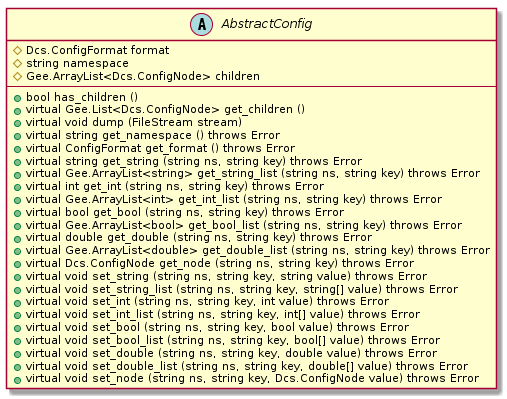
\includegraphics[width=\textwidth]{figures/design/class/core/abstract-config}
          %\caption{Class Diagram for a DcsAbstractConfig}
          \label{fig:dsg-classes-abs-config}
        \end{figure}
      \end{minipage}

      \emph{DcsApplication}

      \vspace*{-0.75cm}
      \begin{minipage}[t]{0.5\textwidth}
        \vspace*{0.5cm}
        Applications in OpenDCS are the base of services as well as GUI and CLI
        processes. Each needs to function as a Model-View-Controller (MVC)
        application in order to have a standardized architecture for plugin
        developers to connect to.
      \end{minipage} \hfill
      \begin{minipage}[t]{0.45\textwidth}
        \begin{figure}[H]
          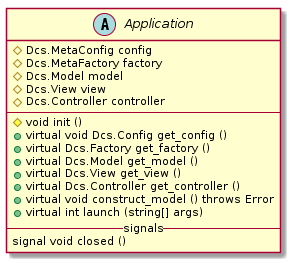
\includegraphics[width=\textwidth]{figures/design/class/core/application}
          %\caption{Class Diagram for a DcsApplication}
          \label{fig:dsg-classes-application}
        \end{figure}
      \end{minipage}

      \emph{DcsConfigNode}

      \vspace*{-0.75cm}
      \begin{minipage}[t]{0.5\textwidth}
        \vspace*{0.5cm}
        Configuration is a core concept of OpenDCS services and applications,
        and central to them is the configuration node. It relates to a single
        configuration object implemented using XML, JSON, and INI key files
        depending on how the configuration file has been implemented. These
        configuration nodes are used by factories to produce node objects which
        form the base of the data model component of the MVC application.
      \end{minipage} \hfill
      \begin{minipage}[t]{0.45\textwidth}
        \begin{figure}[H]
          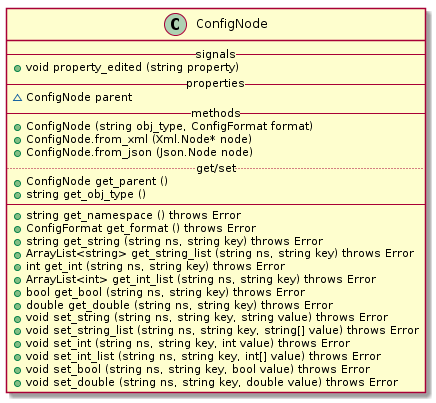
\includegraphics[width=\textwidth]{figures/design/class/core/config-node}
          %\caption{Class Diagram for a DcsConfigNode}
          \label{fig:dsg-classes-config-node}
        \end{figure}
      \end{minipage}

      \emph{DcsConfig}

      \vspace*{-0.75cm}
      \begin{minipage}[t]{0.5\textwidth}
        \vspace*{0.5cm}
        This interface is the generic type which is implemented accross other
        configuration types to provide the contract to use by the developer of
        other configuration types.
      \end{minipage} \hfill
      \begin{minipage}[t]{0.45\textwidth}
        \begin{figure}[H]
          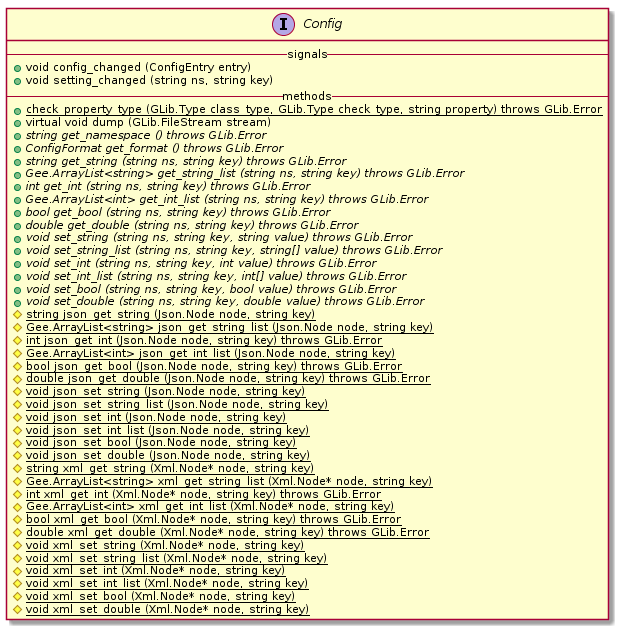
\includegraphics[width=\textwidth]{figures/design/class/core/config}
          %\caption{Class Diagram for a DcsConfig}
          \label{fig:dsg-classes-config}
        \end{figure}
      \end{minipage}

      \emph{DcsController}

      \vspace*{-0.75cm}
      \begin{minipage}[t]{0.5\textwidth}
        \vspace*{0.5cm}
        % TODO provide citation
        A controller in an MVC application is responsible for accepting input
        and converting it to commands for the model or the view.
      \end{minipage} \hfill
      \begin{minipage}[t]{0.45\textwidth}
        \begin{figure}[H]
          \includegraphics[width=\textwidth]{figures/design/class/core/controller}
          %\caption{Class Diagram for a DcsController}
          \label{fig:dsg-classes-controller}
        \end{figure}
      \end{minipage}

      \emph{DcsDataSeries}

      \vspace*{-0.75cm}
      \begin{minipage}[t]{0.5\textwidth}
      	\vspace*{0.5cm}
        A data series within the context of OpenDCS is a building block for
        node objects that need to contain an array of values, some examples of
        this are a feedback controller, a chart trace, or a signal filter.
      \end{minipage} \hfill
      \begin{minipage}[t]{0.45\textwidth}
        \begin{figure}[H]
          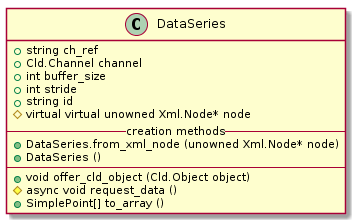
\includegraphics[width=0.6\textwidth]{figures/design/class/core/dataseries}
          %\caption{Class Diagram for a DcsDataSeries}
          \label{fig:dsg-classes-data-series}
        \end{figure}
      \end{minipage}

      \emph{DcsDBusInterface}

      \vspace*{-0.75cm}
      \begin{minipage}[t]{0.5\textwidth}
      	\vspace*{0.5cm}
        In GLib applications DBus interfaces are used by services to create an
        API similar to what would be provided by a REST API. This object is
        carry over from the software that OpenDCS was forked from and will very
        likely find a home in the Net namespace in future versions.
      \end{minipage} \hfill
      \begin{minipage}[t]{0.45\textwidth}
        \begin{figure}[H]
          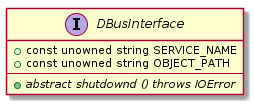
\includegraphics[width=0.8\textwidth]{figures/design/class/core/dbus-interface}
          %\caption{Class Diagram for a DcsDBusInterface}
          \label{fig:dsg-classes-dbus-interface}
        \end{figure}
      \end{minipage}

      \emph{DcsFactory}

      \vspace*{-0.75cm}
      \begin{minipage}[t]{0.5\textwidth}
      	\vspace*{0.5cm}
        Factories in OpenDCS are a means to define a generic way of building
        objects from configuration nodes without having to define a construction
        method within each. It defines the requirements for others implementing
        this on how they need to consume properties and child nodes using the
        parameter specification abilities afforded by GLib objects.
      \end{minipage} \hfill
      \begin{minipage}[t]{0.45\textwidth}
        \begin{figure}[H]
          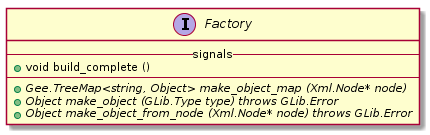
\includegraphics[width=\textwidth]{figures/design/class/core/factory}
          %\caption{Class Diagram for a DcsFactory}
          \label{fig:dsg-classes-factory}
        \end{figure}
      \end{minipage}

      \emph{DcsMessage}

      \vspace*{-0.75cm}
      \begin{minipage}[t]{0.5\textwidth}
      	\vspace*{0.5cm}
        % TODO move to Net
        Messages are a serialized format of an object, or grouping of objects,
        that will be pushed and popped on message queues that are used by
        services to communicate with each other.
      \end{minipage} \hfill
      \begin{minipage}[t]{0.45\textwidth}
        \begin{figure}[H]
          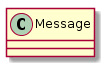
\includegraphics[width=\textwidth]{figures/design/class/core/message}
          %\caption{Class Diagram for a DcsMessage}
          \label{fig:dsg-classes-message}
        \end{figure}
      \end{minipage}

      \emph{DcsMetaConfig}

      \vspace*{-0.75cm}
      \begin{minipage}[t]{0.5\textwidth}
      	\vspace*{0.5cm}
        The meta configuration class provides applications a method of loading
        multiple configurations of various types in at runtime without knowing
        exactly what they provide. It is essentially a list of configuration
        types and methods to iterate over those to get and set objects and
        properties that they provide.
      \end{minipage} \hfill
      \begin{minipage}[t]{0.45\textwidth}
        \begin{figure}[H]
          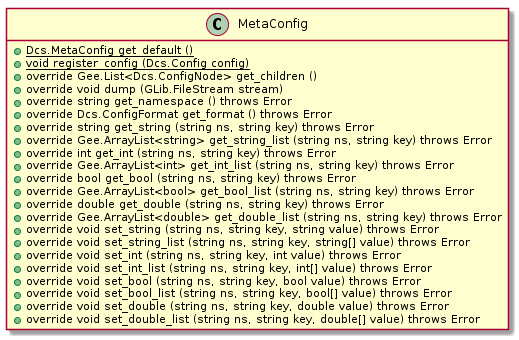
\includegraphics[width=\textwidth]{figures/design/class/core/meta-config}
          %\caption{Class Diagram for a DcsMetaConfig}
          \label{fig:dsg-classes-meta-config}
        \end{figure}
      \end{minipage}

      \emph{DcsMetaFactory}

      \vspace*{-0.75cm}
      \begin{minipage}[t]{0.5\textwidth}
      	\vspace*{0.5cm}
        The meta factory class provides applications a method of loading
        multiple object factories of various types in a runtime without knowing
        what the produce for a given configuration node. It is a list of factory
        types and methods to iterate over those to be used to create object
        nodes that end up in an application's data model.
      \end{minipage} \hfill
      \begin{minipage}[t]{0.45\textwidth}
        \begin{figure}[H]
          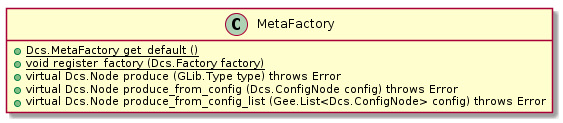
\includegraphics[width=\textwidth]{figures/design/class/core/meta-factory}
          %\caption{Class Diagram for a DcsMetaFactory}
          \label{fig:dsg-classes-meta-factory}
        \end{figure}
      \end{minipage}

      \emph{DcsModel}

      \vspace*{-0.75cm}
      \begin{minipage}[t]{0.5\textwidth}
      	\vspace*{0.5cm}
        % TODO provide citation
        A model in an MVC application stores data that is retrieved using
        commands from the controller and to update what is displayed in the
        view.
      \end{minipage} \hfill
      \begin{minipage}[t]{0.45\textwidth}
        \begin{figure}[H]
          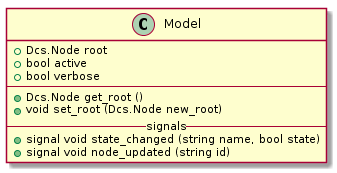
\includegraphics[width=\textwidth]{figures/design/class/core/model}
          %\caption{Class Diagram for a DcsModel}
          \label{fig:dsg-classes-model}
        \end{figure}
      \end{minipage}

      \emph{DcsNode}

      \vspace*{-0.75cm}
      \begin{minipage}[t]{0.5\textwidth}
      	\vspace*{0.5cm}
        The node class is a fundamental component of constructing the data model
        for services, it is extends a tree map ADT and is meant to contain other
        objects that derive it. Nodes have properties, an optional parent, and
        optional children, all of which describe the object and allow it to be
        constructed generically and placed within the data model tree.
      \end{minipage} \hfill
      \begin{minipage}[t]{0.45\textwidth}
        \begin{figure}[H]
          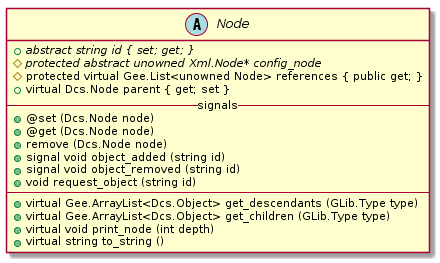
\includegraphics[width=\textwidth]{figures/design/class/core/node}
          %\caption{Class Diagram for a DcsNode}
          \label{fig:dsg-classes-node}
        \end{figure}
      \end{minipage}

      \emph{DcsObject}

      \vspace*{-0.75cm}
      \begin{minipage}[t]{0.5\textwidth}
      	\vspace*{0.5cm}
        An object is the base interface for all classes to implement that work
        across OpenDCS libraries and within service data models.
      \end{minipage} \hfill
      \begin{minipage}[t]{0.45\textwidth}
        \begin{figure}[H]
          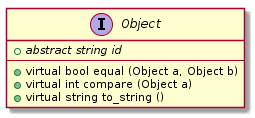
\includegraphics[width=0.8\textwidth]{figures/design/class/core/object}
          %\caption{Class Diagram for a DcsObject}
          \label{fig:dsg-classes-object}
        \end{figure}
      \end{minipage}

      \emph{DcsPluginInformation}

      \vspace*{-0.75cm}
      \begin{minipage}[t]{0.5\textwidth}
      	\vspace*{0.5cm}
        The plugin information class will be used to describe features that the
        plugin provides, for example if a plugin is meant to read values from a
        piece of data acquisition hardware it will provide the values read as
        analog input channels.
      \end{minipage} \hfill
      \begin{minipage}[t]{0.45\textwidth}
        \begin{figure}[H]
          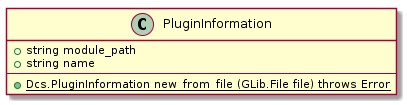
\includegraphics[width=\textwidth]{figures/design/class/core/plugin-information}
          %\caption{Class Diagram for a DcsPluginInformation}
          \label{fig:dsg-classes-plugin-information}
        \end{figure}
      \end{minipage}

      \emph{DcsPluginManager}

      \vspace*{-0.75cm}
      \begin{minipage}[t]{0.5\textwidth}
      	\vspace*{0.5cm}
        In other namespaces plugin managers will use this common class so that
        services have a general base for the functionality the plugin system is
        meant to provide.
      \end{minipage} \hfill
      \begin{minipage}[t]{0.45\textwidth}
        \begin{figure}[H]
          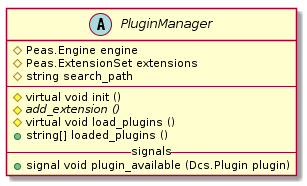
\includegraphics[width=\textwidth]{figures/design/class/core/plugin-manager}
          %\caption{Class Diagram for a DcsPluginManager}
          \label{fig:dsg-classes-plugin-manager}
        \end{figure}
      \end{minipage}

      \emph{DcsPlugin}

      \vspace*{-0.75cm}
      \begin{minipage}[t]{0.5\textwidth}
      	\vspace*{0.5cm}
        A plugin object is the class that other plugin types base off of, it
        defines the basic requirements that libpeas has of plugin extensions.
        All plugins in OpenDCS will additionally have the ability to perform
        some execution in a thread, so the provision for that has been added.
      \end{minipage} \hfill
      \begin{minipage}[t]{0.45\textwidth}
        \begin{figure}[H]
          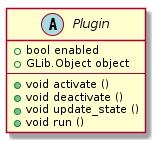
\includegraphics[width=0.5\textwidth]{figures/design/class/core/plugin}
          %\caption{Class Diagram for a DcsPlugin}
          \label{fig:dsg-classes-plugin}
        \end{figure}
      \end{minipage}

      \emph{Point}

      \vspace*{-0.75cm}
      \begin{minipage}[t]{0.5\textwidth}
      	\vspace*{0.5cm}
        Points are a simple class that are used at a variety of locations
        including in measurements, data series value groups, and chart traces
        in the GUI which hasn't been included in this report.
      \end{minipage} \hfill
      \begin{minipage}[t]{0.45\textwidth}
        \begin{figure}[H]
          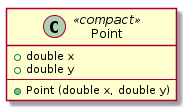
\includegraphics[width=0.6\textwidth]{figures/design/class/core/point}
          %\caption{Class Diagram for a DcsPoint}
          \label{fig:dsg-classes-point}
        \end{figure}
      \end{minipage}

      \emph{DcsRefContainer}

      \vspace*{-0.75cm}
      \begin{minipage}[t]{0.5\textwidth}
      	\vspace*{0.5cm}
        References are an integral part of how the objects contained in a data
        model connect to each other, this class provides the ability to work
        with those references in a safe manner.
      \end{minipage} \hfill
      \begin{minipage}[t]{0.45\textwidth}
        \begin{figure}[H]
          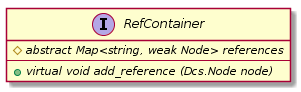
\includegraphics[width=\textwidth]{figures/design/class/core/ref-container}
          %\caption{Class Diagram for a DcsRefContainer}
          \label{fig:dsg-classes-ref-container}
        \end{figure}
      \end{minipage}

      \emph{DcsRefLinker}

      \vspace*{-0.75cm}
      \begin{minipage}[t]{0.5\textwidth}
      	\vspace*{0.5cm}
        Reference linking is performed by an application after every time new
        references have been added to an object. This object uses the singleton
        pattern as it contains data about the entire application and would
        present problems if multiple instances existed.
      \end{minipage} \hfill
      \begin{minipage}[t]{0.45\textwidth}
        \begin{figure}[H]
          \includegraphics[width=\textwidth]{figures/design/class/core/ref-linker}
          %\caption{Class Diagram for a DcsRefLinker}
          \label{fig:dsg-classes-ref-linker}
        \end{figure}
      \end{minipage}

      \emph{DcsSerializable}

      \vspace*{-0.75cm}
      \begin{minipage}[t]{0.5\textwidth}
      	\vspace*{0.5cm}
        This interface is used by objects that will need to be serialized and
        deserialized for the purpose of passing across networks using ZeroMQ and
        REST messaging.
      \end{minipage} \hfill
      \begin{minipage}[t]{0.45\textwidth}
        \begin{figure}[H]
          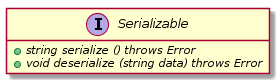
\includegraphics[width=0.8\textwidth]{figures/design/class/core/serializable}
          %\caption{Class Diagram for a DcsSerializable}
          \label{fig:dsg-classes-serializable}
        \end{figure}
      \end{minipage}

      \emph{DcsSyslog}

      \vspace*{-0.75cm}
      \begin{minipage}[t]{0.5\textwidth}
      	\vspace*{0.5cm}
        The logging facility provides a format for output strings and controls
        what level of messages will be output based on a variable controlling
        verbosity. It provides control to the user over the output depending on
        whether they want to see minimal messages all the way up to very
        verbose debugging and trace messages.
      \end{minipage} \hfill
      \begin{minipage}[t]{0.45\textwidth}
        \begin{figure}[H]
          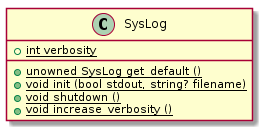
\includegraphics[width=0.8\textwidth]{figures/design/class/core/syslog}
          %\caption{Class Diagram for a DcsSyslog}
          \label{fig:dsg-classes-syslog}
        \end{figure}
      \end{minipage}

      \emph{DcsView}

      \vspace*{-0.75cm}
      \begin{minipage}[t]{0.5\textwidth}
      	\vspace*{0.5cm}
        A view in an MVC application is used to generate new output based on
        changes to the model.
      \end{minipage} \hfill
      \begin{minipage}[t]{0.45\textwidth}
        \begin{figure}[H]
          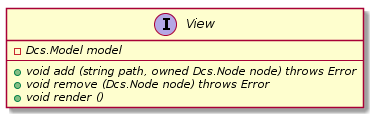
\includegraphics[width=\textwidth]{figures/design/class/core/view}
          %\caption{Class Diagram for a DcsView}
          \label{fig:dsg-classes-view}
        \end{figure}
      \end{minipage}

    \subsubsection{Data Acquisition Library}\label{sec:dsg-classes-daq}

      Classes in the DAQ library will provide the functionality required to
      create objects that communicate with physical devices. Plugins in this
      namespace are referred to as devices, these device plugins are meant to be
      created to read and write real world values and present them over the
      message queueing systems available.

      \emph{DcsDaqDeviceManager}

      \vspace*{-0.75cm}
      \begin{minipage}[t]{0.5\textwidth}
      	\vspace*{0.5cm}
        The device manager class is the DAQ namespace specific implementation of
        the plugin manager to be used by services and applications that want to
        load hardware device type plugins.
      \end{minipage} \hfill
      \begin{minipage}[t]{0.45\textwidth}
        \begin{figure}[H]
          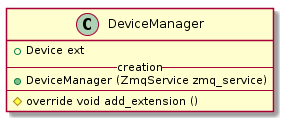
\includegraphics[width=0.8\textwidth]{figures/design/class/daq/device-manager}
          %\caption{Class Diagram for a DcsDaqDeviceManager}
          \label{fig:dsg-classes-daq-device-manager}
        \end{figure}
      \end{minipage}

      \emph{DcsDaqDevice}

      \vspace*{-0.75cm}
      \begin{minipage}[t]{0.5\textwidth}
      	\vspace*{0.5cm}
        This serves as a base for any device plugins that will be developed and
        loaded by services and applications that contain a device manager.
      \end{minipage} \hfill
      \begin{minipage}[t]{0.45\textwidth}
        \begin{figure}[H]
          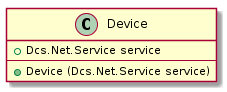
\includegraphics[width=0.6\textwidth]{figures/design/class/daq/device}
          %\caption{Class Diagram for a DcsDaqDevice}
          \label{fig:dsg-classes-daq-device}
        \end{figure}
      \end{minipage}

      \emph{DcsDaqFactory}

      \vspace*{-0.75cm}
      \begin{minipage}[t]{0.5\textwidth}
      	\vspace*{0.5cm}
        The factory class in this namespace serves the same function as other
        factories, except that it produces DAQ specific objects. It is meant to
        be used with the DcsMetaFactory class as part of a larger application.
      \end{minipage} \hfill
      \begin{minipage}[t]{0.45\textwidth}
        \begin{figure}[H]
          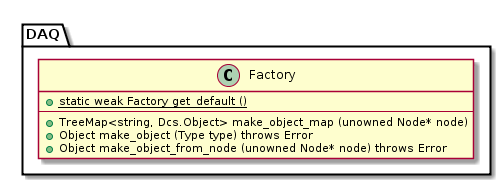
\includegraphics[width=\textwidth]{figures/design/class/daq/factory}
          %\caption{Class Diagram for a DcsDaqFactory}
          \label{fig:dsg-classes-daq-factory}
        \end{figure}
      \end{minipage}

    \subsubsection{Data Logging Library}\label{sec:dsg-classes-log}

      Classes in the data logging library will provide the functionality
      required to read and write data values that it has received into any
      format that has been defined by the plugins. Plugins in this namespace are
      referred to as backends, these logging plugins are meant to create and
      work with different file formats, databases, and whatever else makes sense
      to record data onto.

      \emph{DcsLogBackendManager}

      \vspace*{-0.75cm}
      \begin{minipage}[t]{0.5\textwidth}
      	\vspace*{0.5cm}
        The backend manager class is the Log namespace specific implementation
        of the plugin manager to be used by services and applications that want
        to load logging backend type plugins.
      \end{minipage} \hfill
      \begin{minipage}[t]{0.45\textwidth}
        \begin{figure}[H]
          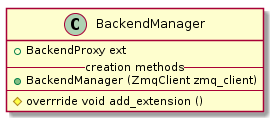
\includegraphics[width=0.8\textwidth]{figures/design/class/log/backend-manager}
          %\caption{Class Diagram for a DcsLogBackendManager}
          \label{fig:dsg-classes-log-backend-manager}
        \end{figure}
      \end{minipage}

      \emph{DcsLogBackend}

      \vspace*{-0.75cm}
      \begin{minipage}[t]{0.5\textwidth}
      	\vspace*{0.5cm}
        This serves as a base for any backend plugin that will be developed and
        loaded by services and applications that contain a backend manager.
      \end{minipage} \hfill
      \begin{minipage}[t]{0.45\textwidth}
        \begin{figure}[H]
          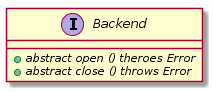
\includegraphics[width=0.6\textwidth]{figures/design/class/log/backend}
          %\caption{Class Diagram for a DcsLogBackend}
          \label{fig:dsg-classes-log-backend}
        \end{figure}
      \end{minipage}

      \emph{DcsLogFactory}

      \vspace*{-0.75cm}
      \begin{minipage}[t]{0.5\textwidth}
      	\vspace*{0.5cm}
        The factory class in this namespace serves the same function as other
        factories, except that it produces Log specific objects. It is meant to
        be used with the DcsMetaFactory class as part of a larger application.
      \end{minipage} \hfill
      \begin{minipage}[t]{0.45\textwidth}
        \begin{figure}[H]
          \includegraphics[width=\textwidth]{figures/design/class/log/factory}
          %\caption{Class Diagram for a DcsLogFactory}
          \label{fig:dsg-classes-log-factory}
        \end{figure}
      \end{minipage}

    \subsubsection{Feedback Control Library}\label{sec:dsg-classes-ctl}

      Classes in the feedback control library will provide the functionality
      required to
      read and write data values that it has received into any
      format that has been defined by the plugins. Plugins in this namespace are
      referred to as backends, these logging plugins are meant to create and
      work with different file formats, databases, and whatever else makes sense
      to record data onto

      \emph{DcsControlControllerManager}

      \vspace*{-0.75cm}
      \begin{minipage}[t]{0.5\textwidth}
      	\vspace*{0.5cm}
        The controller manager class is the Control namespace specific
        implementation of the plugin manager to be used by services and
        applications that want to load feedback controller type plugins.
      \end{minipage} \hfill
      \begin{minipage}[t]{0.45\textwidth}
        \begin{figure}[H]
          \includegraphics[width=0.8\textwidth]{figures/design/class/control/controller-manager}
          \label{fig:dsg-classes-control-controller-manager}
        \end{figure}
      \end{minipage}

      \emph{DcsControlController}

      \vspace*{-0.75cm}
      \begin{minipage}[t]{0.5\textwidth}
      	\vspace*{0.5cm}
        This serves as a base for any controller plugin that will be developed
        and loaded by services and applications that contain a controller
        manager.
      \end{minipage} \hfill
      \begin{minipage}[t]{0.45\textwidth}
        \begin{figure}[H]
          \includegraphics[width=0.6\textwidth]{figures/design/class/control/controller}
          \label{fig:dsg-classes-control-controller}
        \end{figure}
      \end{minipage}

      \emph{DcsControlFactory}

      \vspace*{-0.75cm}
      \begin{minipage}[t]{0.5\textwidth}
      	\vspace*{0.5cm}
        The factory class in this namespace serves the same function as other
        factories, except that it produces Control specific objects. It is
        meant to be used with the DcsMetaFactory class as part of a larger
        application.
      \end{minipage} \hfill
      \begin{minipage}[t]{0.45\textwidth}
        \begin{figure}[H]
          \includegraphics[width=\textwidth]{figures/design/class/control/factory}
          \label{fig:dsg-classes-control-factory}
        \end{figure}
      \end{minipage}

    \subsubsection{Networking Library}\label{sec:dsg-classes-net}

      The networking library contains classes that are used to communicate with
      other services. This ability is accomplished using ZeroMQ and REST as the
      messaging systems, but is left open for others such as DBus or RabbitMQ.

      \emph{DcsNetFactory}

      \vspace*{-0.75cm}
      \begin{minipage}[t]{0.5\textwidth}
      	\vspace*{0.5cm}
        The factory class in this namespace serves the same function as other
        factories, except that it produces Net specific objects. It is meant to
        be used with the DcsMetaFactory class as part of a larger application.
      \end{minipage} \hfill
      \begin{minipage}[t]{0.45\textwidth}
        \begin{figure}[H]
          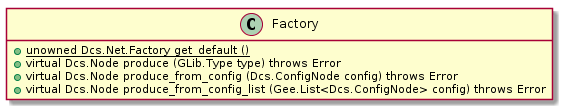
\includegraphics[width=\textwidth]{figures/design/class/net/factory}
          %\caption{Class Diagram for a DcsNetFactory}
          \label{fig:dsg-classes-net-factory}
        \end{figure}
      \end{minipage}

      \emph{DcsNetService}

      \vspace*{-0.75cm}
      \begin{minipage}[t]{0.5\textwidth}
      	\vspace*{0.5cm}
        Services are an extension of applications and use the same MVC design
        pattern, but they add the concept of plugin systems and expose features
        that are required by plugins to function as part of the system.
      \end{minipage} \hfill
      \begin{minipage}[t]{0.45\textwidth}
        \begin{figure}[H]
          \includegraphics[width=\textwidth]{figures/design/class/net/service}
          %\caption{Class Diagram for a DcsNetService}
          \label{fig:dsg-classes-net-service}
        \end{figure}
      \end{minipage}

      \emph{DcsNetRestService}

      \vspace*{-0.75cm}
      \begin{minipage}[t]{0.5\textwidth}
      	\vspace*{0.5cm}
        This is an abstract base that service implementations must extend and
        define if they want to provide a RESTful API. It exists mainly to be
        added as a contract to the DcsNetService class to ensure services
        include one.
      \end{minipage} \hfill
      \begin{minipage}[t]{0.45\textwidth}
        \begin{figure}[H]
          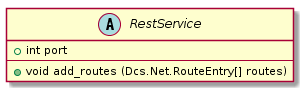
\includegraphics[width=0.8\textwidth]{figures/design/class/net/rest-service}
          %\caption{Class Diagram for a DcsNetRestService}
          \label{fig:dsg-classes-net-rest-service}
        \end{figure}
      \end{minipage}

      \emph{DcsNetPublish}

      \vspace*{-0.75cm}
      \begin{minipage}[t]{0.5\textwidth}
      	\vspace*{0.5cm}
        A publish object makes a connection to a ZeroMQ context and provides a
        means of configuring this type of socket using the configuration and
        production methods of this project.
      \end{minipage} \hfill
      \begin{minipage}[t]{0.45\textwidth}
        \begin{figure}[H]
          \includegraphics[width=0.8\textwidth]{figures/design/class/net/publish}
          %\caption{Class Diagram for a DcsNetPublish}
          \label{fig:dsg-classes-net-publish}
        \end{figure}
      \end{minipage}

      \emph{DcsNetSubscribe}

      \vspace*{-0.75cm}
      \begin{minipage}[t]{0.5\textwidth}
      	\vspace*{0.5cm}
        A subscribe object makes a connection to a ZeroMQ context and provides a
        means of configuring this type of socket using the configuration and
        production methods of this project.
      \end{minipage} \hfill
      \begin{minipage}[t]{0.45\textwidth}
        \begin{figure}[H]
          \includegraphics[width=\textwidth]{figures/design/class/net/subscribe}
          %\caption{Class Diagram for a DcsNetSubscribe}
          \label{fig:dsg-classes-net-subscribe}
        \end{figure}
      \end{minipage}

      \emph{DcsNetRequest}

      \vspace*{-0.75cm}
      \begin{minipage}[t]{0.5\textwidth}
      	\vspace*{0.5cm}
        A request object makes a connection to a ZeroMQ context and provides a
        means of configuring this type of socket using the configuration and
        production methods of this project.
      \end{minipage} \hfill
      \begin{minipage}[t]{0.45\textwidth}
        \begin{figure}[H]
          \includegraphics[width=0.8\textwidth]{figures/design/class/net/request}
          %\caption{Class Diagram for a DcsNetRequest}
          \label{fig:dsg-classes-net-request}
        \end{figure}
      \end{minipage}

      \emph{DcsNetReply}

      \vspace*{-0.75cm}
      \begin{minipage}[t]{0.5\textwidth}
      	\vspace*{0.5cm}
        A reply object makes a connection to a ZeroMQ context and provides a
        means of configuring this type of socket using the configuration and
        production methods of this project.
      \end{minipage} \hfill
      \begin{minipage}[t]{0.45\textwidth}
        \begin{figure}[H]
          \includegraphics[width=0.8\textwidth]{figures/design/class/net/reply}
          %\caption{Class Diagram for a DcsNetReply}
          \label{fig:dsg-classes-net-reply}
        \end{figure}
      \end{minipage}

  \subsection{Class Diagrams}\label{sec:dsg-class-dia}

    Using the objects defined in Section~\ref{sec:dsg-classes} this section will
    define the structure of the core components of how the services will be
    constructed. These consist of configurations, object factories to produce
    generic objects using configuration nodes, plugins, and services or
    applications.

    \emph{Configuration Composition}

    OpenDCS services are based on a concept of being configurable at many
    levels, the diagram provided for the service configuration composition
    in Figure~\ref{fig:dsg-class-config} shows how the constituent
    classes are organized. At the top level the service contains a single
    configuration class \emph{Dcs.MetaConfig} that itself contains all of
    the other configurations regardless of type and it is used by the
    service as a single point into the group. This design allows for
    a variety of configuration concepts including variables set during
    launch using command line arguments, files loaded from the system,
    and partial configuration files loaded by the plugins during setup.

    \begin{figure}[H]
      \includegraphics[width=\textwidth]{figures/design/class/config}
      \caption{Class Diagram for the Configuration Composition}
      \label{fig:dsg-class-config}
    \end{figure}

    \emph{Object Factory Composition}

    Much like the configuration concept, the services have a single point for
    application access which is shown in Figure~\ref{fig:dsg-class-factory}.
    With this component the factories consume \emph{Dcs.ConfigNode} objects
    and produce \emph{Dcs.Node} objects which form the data model that is used
    by the entire service or application. It is meant to do this in a very
    generic fashion where each namespace is responsible for providing the
    objects that they know of, as well as a method to allow plugins which are
    completely unknown to the service the ability to construct new objects that
    will integrate with the system.

    \begin{figure}[H]
      \includegraphics[width=\textwidth]{figures/design/class/factory}
      \caption{Class Diagram for the Object Factory Composition}
      \label{fig:dsg-class-factory}
    \end{figure}

    \emph{Plugin System Composition}

    The plugin system is the next fundamental component of the design and in
    it the idea is to have each namespace define a manager and plugins of their
    own type, these are then used with any service that wants to implement that
    form of plugin. While this could have been implemented as a single plugin
    manager and plugin type this is intended to allow for a more logical means
    of installing and managing plugins when installed on a host. Core to these
    plugins is the ability to access the service application and what it
    provides, and more specifically the model, view, and controller (MVC) of
    that process. Having access to the MVC means that the plugin can attach new
    objects to the data model providing they follow the standard format, to add
    new view components that are rendered to an end user, and to communicate
    with the abilities of the service through the controller.

    \begin{figure}[H]
      \includegraphics[width=\textwidth]{figures/design/class/plugin}
      \caption{Class Diagram for the Plugin System Composition}
      \label{fig:dsg-class-plugin}
    \end{figure}

    \emph{Service/Application Composition}

    Services, or applications, are the final piece that bring together the
    other concepts presented in this section. They are responsible for loading
    all plugins during launch, reading and combining all configurations,
    producing the data model using the aggregated object factories, and
    providing the plugins with what they require to put messages onto the
    message queues of the service that are wired up with other services.

    \begin{figure}[H]
        \includegraphics[width=\textwidth]{figures/design/class/service}
      \caption{Class Diagram for the Service/Application Composition}
      \label{fig:dsg-class-service}
    \end{figure}

  \subsection{Sequence Diagrams}\label{sec:dsg-sequence}

    The project life cycle sequence does not impact the development of this
    software, but it is important to the client that they understand how it
    would affect their workflow. Figure~\ref{fig:dsg-sequence-life-cycle} shows
    a proposed method without getting into the specifics of configuration. As
    that is a somewhat complicated task that requires knowledge of the system as
    well the configuration language used, XML and JSON, it would take
    significant effort to adequately describe and is outside of the scope of
    this document.

    \begin{figure}[H]
      \includegraphics[width=0.8\textwidth,center]{figures/design/sequence/project-lifecycle}
      \caption{Project Life Cycle Sequence Diagram}
      \label{fig:dsg-sequence-life-cycle}
    \end{figure}

    All of the services that will be developed as part of OpenDCS rely heavily
    on the usage of plugins, as such it is worthwhile to outline how the generic
    service concept will go about loading plugins from the file system. What is
    not described in Figure~\ref{fig:dsg-sequence-load-plugins} is how to create
    a plugin, or where the system expects them to reside. This information will
    be given later on in Section~\ref{sec:inst}.

    \begin{figure}[H]
      \includegraphics[width=0.8\textwidth,center]{figures/design/sequence/load-plugins}
      \caption{Plugin Loading Sequence Diagram}
      \label{fig:dsg-sequence-load-plugins}
    \end{figure}

    The next three sequence diagrams show the process sequence of key concepts.
		Figure~\ref{fig:dsg-sequence-measure-request} is meant to describe what
		should happen when a user of the system requests a measurement from the DAQ
    service, Figure~\ref{fig:dsg-sequence-query-request} for a data query of
    the logging service, and Figure~\ref{fig:dsg-sequence-control-request} for
    a process control change of the feedback control service.

    A measurement in OpenDCS is performed by a device plugin, the DAQ service
    itself is only responsible for loading the plugin and providing the
    connection between the device and the messaging system that other services
    and applications communicate to it through. In the case of a request-reply
    type request made by the end user where a measurement is requested and the
    measured value is provided in a reply the sequence follows this pattern.

    \begin{figure}[H]
      \includegraphics[width=\textwidth]{figures/design/sequence/measure-request}
      \caption{Data Acquisition Service Measurement Sequence Diagram}
      \label{fig:dsg-sequence-measure-request}
    \end{figure}

    Logging services, like the DAQ service, do the bulk of the actual work
    through plugins that communicate with underlying files and databases
    depending on what they've been developed to use. The pattern used by users
    of the service always follow a request-reply sequence where the user acting
    on the service makes a query request that defines a date and time range that
    they are interested in and the service provides the result as a formatted
    data set.

    \begin{figure}[H]
      \includegraphics[width=\textwidth]{figures/design/sequence/query-request}
      \caption{Data Log Service Query Sequence Diagram}
      \label{fig:dsg-sequence-query-request}
    \end{figure}

    Lastly, the feedback control service, again like the DAQ service, does its
    work using plugins that receive data from the DAQ service, perform and
    calculation in a controller plugin and feed the change back to the DAQ
    service to perform the actual work. The sequence given here is that of a
    single change request being made by the user, in reality the interaction
    between the control and DAQ services would take place several times and
    would not necessarily be done over a request-reply socket pair, but for
    brevity this is how it's been illustrated.

    \begin{figure}[H]
      \includegraphics[width=\textwidth]{figures/design/sequence/control-request}
      \caption{Feedback Controller Service Change Sequence Diagram}
      \label{fig:dsg-sequence-control-request}
    \end{figure}

  \subsection{Component Diagrams}\label{sec:dsg-component}

    OpenDCS is a service oriented architecture where each should be developed to
    very similar to the others. The standard component format is shown in
    Figure~\ref{fig:dsg-component-service}, this provides a very high level
    outline of the intended way for a service to be constructed to provide a way
    for external applications to communicate with it.

    \begin{figure}[H]
      \includegraphics[width=\textwidth]{figures/design/component/service}
      \caption{Service Component Diagram}
      \label{fig:dsg-component-service}
    \end{figure}

    Additionally, the services will all be designed to implement a plugin
    manager system so that a common framework for plugins can be utilized. This
    framework is given in Figure~\ref{fig:dsg-component-plugin} which
    illustrates how plugins are loaded and what they should provide. The term
    ``Meta'' is used to describe that the configuration and factory components
    of services are constructed of multiples of the same type across the various
    namespaces.

    \begin{figure}[H]
      \includegraphics[width=\textwidth]{figures/design/component/plugin}
      \caption{Plugin Component Diagram}
      \label{fig:dsg-component-plugin}
    \end{figure}
